\documentclass{article} %[twoside]
\usepackage{relsize,epsfig,makeidx,amsmath,amsfonts,listings,color}
\usepackage[latin1]{inputenc}
\usepackage{changepage}
\usepackage{a4wide}
\usepackage{filecontents}
\begin{filecontents}{\jobname.bib}
@Manual{proj2,
title = {project2_2013},
OPTkey = {•},
OPTauthor = {•},
OPTorganization = {•},
OPTaddress = {•},
OPTedition = {•},
OPTmonth = {•},
OPTyear = {2013},
note = {Project description for project 2 in FYS4150},
OPTannote = {•}
}

\end{filecontents}
\immediate\write18{bibtex \jobname}


% Hyperlinks in PDF:
\usepackage[colorlinks=true,linkcolor=black,citecolor=black,
    filecolor=black,urlcolor=black,pdfmenubar=true,pdftoolbar=true,
    urlcolor=black,bookmarksdepth=3]{hyperref}
\newcommand*\tageq{\refstepcounter{equation}\tag{\theequation}}

\definecolor{gray}{rgb}{0.3,0.3,0.3}
\definecolor{dgreen}{rgb}{0.0,0.5,0.0}

\lstset{ %
  backgroundcolor=\color{white},   	% choose the background color; you must add \usepackage{color} or \usepackage{xcolor}
  basicstyle=\footnotesize,        	% the size of the fonts that are used for the code
  breakatwhitespace=false,         	% sets if automatic breaks should only happen at whitespace
  breaklines=true,                 	% sets automatic line breaking
  captionpos=b,                    	% sets the caption-position to bottom
  commentstyle=\color{dgreen},    	% comment style
  deletekeywords={...},            	% if you want to delete keywords from the given language
  escapeinside={\%*}{*)},          	% if you want to add LaTeX within your code
  extendedchars=true,              	% lets you use non-ASCII characters; for 8-bits encodings only, does not work with UTF-8
  frame=single,                    		% adds a frame around the code
  keepspaces=true,                 	% keeps spaces in text, useful for keeping indentation of code (possibly needs columns=flexible)
  keywordstyle=\color{blue},       	% keyword style
  language=C++,			                 	% the language of the code
  morekeywords={self,...},          % if you want to add more keywords to the set
  numbers=left,                    	% where to put the line-numbers; possible values are (none, left, right)
  numbersep=5pt,                   	% how far the line-numbers are from the code
  numberstyle=\tiny\color{gray}, 	% the style that is used for the line-numbers
  rulecolor=\color{black},         	% if not set, the frame-color may be changed on line-breaks within not-black text (e.g. comments (green here))
  showspaces=false,                	% show spaces everywhere adding particular underscores; it overrides 'showstringspaces'
  showstringspaces=false,          	% underline spaces within strings only
  showtabs=false,                  	% show tabs within strings adding particular underscores
  stepnumber=2,                    	% the step between two line-numbers. If it's 1, each line will be numbered
  stringstyle=\color{green},     	% string literal style
  tabsize=2,                       	% sets default tabsize to 2 spaces
  %title=\lstname                   % show the filename of files included with \lstinputlisting; also try caption instead of title
}
\makeindex


\begin{document}
\title{FYS4150: Project 2}
\author{Mikael Toresen \\
	Robert Fauli}
\date{\today}
\maketitle
\begin{abstract}
In this project we rewrite the three dimensional Schr\"{o}dinger equation for a harmonic oscillator well to get it on a dimesionless form, which can be used to solve the equation for a general case. We furthermore find the dimensionless Schr\"{o}dinger equation for 2 electrons in a harmonic oscillator well with coloumb interaction. This is then solved numerically using the Jacobi method to solve the equation as an eigenvalue problem and comparing results with Armadillos built-in functions. The final part of the project involves looking at the effects that changing a potential parameter has on the eigenvalues and eigenvectors, and its physical interpretation.
%spherically symmetric three-dimensional harmonic oscillator well w/ & w/o coulomb interaction=> eigenvalue equation
%solved with Jacobi's method %(own written code to implement Jacobi's method)
\end{abstract}
\section{Discretizing the problem}\label{s:disc}
\subsection{The dimensionless Schr\"{o}dinger equation}\label{ss:dimlSE}
The general Schr\"{o}dinger equation(SE) can be written as:
\begin{equation}\label{eq:Schr}
	-\frac{\hbar^2}{2m}\frac{{\rm d}\Psi}{{\rm d}\mathbf{x}}+V\Psi = E\Psi
\end{equation}
where $\Psi$ is the wave function, $V$ is the potential and $E$ is the energy.
The radial equation of the SE $R(r)$ for one electron with a harmonic oscillator potential $V=(1/2)kr^2$ where $k=m\omega^2$ is:
\begin{equation}\label{eq:radSE}
	-\frac{\hbar^2}{2m}\left(\frac{1}{r^2}\frac{\mathrm{d}}{\mathrm{d}r}r^2\frac{\mathrm{d}}{\mathrm{d}r}-\frac{l(l+1)}{r^2}\right)R(r)+V(r)R(r)=ER(r)
\end{equation}
with energy levels: \[E_{nl}=\hbar\omega\left(2n+l+\frac{3}{2}\right)\quad n\in\mathbb{N}, \,l\in[0,n)\] where $n$ is the principal quantum number and the quantum number $l$ corresponds to the orbital momentum of the electron. 
We are interested in rewriting the SE using dimensionless variables. If we set $l=0$, substitute $R=u(r)/r$ and rewrite using the dimensionless variable $\rho=r/\alpha$, where $\alpha$ is a constant with dimension length, we arrive at:
\begin{align}
	-\frac{\hbar^2}{2m}\frac{\mathrm{d^2}}{\mathrm{d}\rho}u(\rho)+\left(\frac{k}{2}\alpha^2\rho^2-\frac{l(l+1)}{\rho^2}\frac{\hbar^2}{2m\alpha^2}\right)u(\rho)
	&=Eu(\rho)\\
	%
	-\frac{\hbar^2}{2m}\frac{\mathrm{d^2}}{\mathrm{d}\rho}u(\rho)+\frac{mk}{\hbar^2}\alpha^4\rho^2u(\rho)
	&=\frac{2m\alpha^2}{\hbar^2}\\
	%
	\label{eq:dimlSE}
	-\frac{\mathrm{d^2}}{\mathrm{d}\rho}u(\rho)+\rho^2u(\rho)
	&=\lambda u(\rho)
\end{align}
where 
\[
	\alpha\equiv\left(\frac{\hbar^2}{mk}\right)^{\frac{1}{4}},\quad
	\lambda\equiv\frac{2m\alpha^2}{\hbar^2}E
\]
Equation \eqref{eq:dimlSE} is the dimensionless radial SE for a harmonic oscillator with one electron.

We can similarily use the SE on a similar radial function $u(r_1,r_2)$ to arrive at an expression for two electrons.
This can be rewritten using relative($\mathbf{r}=\mathbf{r}_1-\mathbf{r}_2$ and center-of-mass coordinates($\mathbf(R)=(\mathbf{r}_1+\mathbf{r}_2)/2$:
\begin{align}\label{eq:SE2e}
	\left(-\frac{\hbar^2}{2m}\frac{\mathrm{d^2}}{\mathrm{d}r_1^2} -\frac{\hbar^2}{2m}\frac{\mathrm{d^2}}{\mathrm{d}r^2}
	\frac{k}{2}r_1^2+\frac{k}{2}r_2^2\right)u(r_1,r_2)&=E^{(2)}u(r_1,r_2)\\
	%
	\label{eq:SE2eCMREL}
	\left(-\frac{\hbar^2}{m}\frac{\mathrm{d^2}}{\mathrm{d}r^2} -\frac{\hbar^2}{4m}\frac{\mathrm{d^2}}{\mathrm{d}R^2}
	\frac{k}{4}r^2+kR^2\right)u(r,R)&=E^{(2)}u(r,R)
\end{align}
where $E^{(2)}$ is the energy for two electrons. Equation \eqref{eq:SE2eCMREL} can be decomposed in the same way the radial equation was decomposed from the spherical equation: $u(r,R)=\psi(r)\phi(R)$ and the energy: $E^{(2)}=E_r+E_R$. One can add a repulsive term ($\beta e^2/r$, where $\beta e^2=1.44$eVnm) to the relative equation. This again can be made dimensionless in the same way as to arrive at equation \eqref{eq:dimlSE}:
\begin{equation}\label{eq:dimlSE2e}
	-\frac{\mathrm{d^2}}{\mathrm{d}\rho}\psi(\rho)+\omega_r^2\rho^2\psi(\rho)+\frac{1}{\rho}\psi(\rho)
	=\lambda \psi(\rho)
\end{equation}
where 
\[
	\omega^2_r\equiv\frac{1}{4}\frac{mk}{\hbar^2}\alpha^4,\quad\alpha\equiv\frac{\hbar^2}{m\beta e^2},\quad \lambda=\frac{m\alpha^2}{\hbar^2}E
\]

\subsection{The discrete Schr\"{o}dinger equation}\label{ss:discSE}
We discretize this equation to a mesh with points $\rho_i=\rho_{min}+ih,\, i\in[0,n_{step}]$ where $h$ is defined as $h=(\rho_{max}-\rho_{min})/n_{step}$. 
The second derivative of a function $u$ can approximated by 
$({u_{i+1}-u_i+u_{i-1}})/({h^2})$, where $u_i=u(\rho_i)$. The potential can be written as $V_i=\rho_i^2$. Putting this together we can write the discretized version of equation \eqref{eq:dimlSE} as:
\begin{equation}\label{eq:dimlSEdisc}
	\frac{u_{i+1}-2u_i+u_{i-1}}{h^2} + V_iu_i^2=\lambda u_i
\end{equation}

This can be written as a tridiagonal matrix eigenvalue problem with diagonals $d_i=2h^{-2}+V_i$ and off diagonal elements $e_i=-h^{-2}$:
\begin{equation}\label{eq:matrix}
	\begin{pmatrix}
d_1 	& e_1 	& 0 	& \cdots 	& \cdots 	& 0\\
e_1 	& d_2 	& e_2	& 0				&					&\vdots\\
0 		& e_2 	& d_3 & e_3 		& 0 			&\vdots		\\ 
\vdots & \ddots &\ddots &\ddots &\ddots&\vdots\\
\vdots & 			&0		& e_{n_{step}-2} & d_{n_{step}-2} & e_{n_{step}-1}\\
0 		&\cdots &\cdots& 0 			& e_{n_{step}-1}& \vphantom{\vdots}d_{n_{step}-1} 
\end{pmatrix}
\begin{pmatrix}
u_1\vphantom{0}\\u_2\vphantom{\vdots}\\u_3\vphantom{\vdots}\\ \vdots\\u_{n-1}\vphantom{\vdots}\\u_n\vphantom{\vdots}
\end{pmatrix}
=\lambda
\begin{pmatrix}
u_1\vphantom{0}\\ u_2\vphantom{\vdots}\\ u_3\vphantom{\vdots}\\ \vdots\vphantom{\vdots}\\u_{n-1}\vphantom{\vdots}\\ u_n\vphantom{\vdots}
\end{pmatrix}
\end{equation}

%
Similarily, for the equation for two electrons in a harmonic oscillator interacting via Coulomb interation	using relative coordinates can also be written on the form given in equation \eqref{eq:dimlSE} where the potential now is $V_i=\omega_r^2\rho_i^2+\rho_i^{-1}$. To avoid a zero-division we can no longer use $\rho_{min}=0$.

\subsection{Jacobi's method}\label{ss:jacobi}
Jacobi's method is based on a set of similarity transformations $\mathbf{B}=\mathbf{S}^T\mathbf{A}\mathbf{S}$ where $\mathbf{S}^T=\mathbf{S}^{-1}$. 
The matrix $\mathbf{S}$ can be interpreted geometrically as a rotation of the ($kl$-)plane by an angle $\theta$ and will have a form similar to an identity matrix except for in 4 matrix elements, $s_{kk}=s_{ll}=\cos\theta,\,s_{kl}=-s_{lk}=-\sin\theta$.
$\mathbf{B}$'s elements will be of the form:
\begin{align*}
	b_{ii}	&=	a_{ii},\, i\ne k,\,i\ne l\\
	b_{ik}	&=	a_{ik}\cos\theta - 	a_{il}\sin\theta,\, i\ne k,\,i\ne l\\
	b_{il}	&=	a_{il}\cos\theta + a_{ik}\sin\theta,\, i\ne k,\,i\ne l\\
	b_{kk}	&=	a_{kk}\cos^2\theta - 2a_{kl}\cos\theta\sin\theta + a_{ll}\sin^2\theta\\
	b_{ll}	&= 	a_{ll}\cos^2\theta + 2a_{kl}\cos\theta\sin\theta + a_{kk}\sin^2\theta\\
	b_{kl}	&= 	(a_{kk}-a_{ll})\cos\theta\sin\theta + a_{kl}(\cos^2\theta-\sin^2\theta)	
\end{align*}

By continually finding the largest off-diagonal matrix element given by 
\[
	\text{off}(\mathbf{A})=\sqrt{\sum_{i=1}^n\sum_{j\ne i}^n a_{ij}^2}
\]
and performing the similarity transformations where $k$ and $l$ are its indices, it can be shown that the matrix will tend towards a diagonal form.

To do this then have to set $\theta$ such that the off-diagonal terms become $b_{kl}=0$.

If we define $\tan\theta\equiv t=s/c$, where $s=\sin\theta,\,c=\cos\theta$ and 

we can find an expression for $s$ and $c$ by inserting for the expression for $b_{kl}$ and evaluating the quadratic equation:
\begin{align*}	
	0&= 	(a_{kk}-a_{ll})\cos\theta\sin\theta + a_{kl}(\cos^2\theta-\sin^2\theta)	\\
	&=\frac{a_{kk}-a_{ll}}{2a_{kl}}\cos\theta\sin\theta+\frac{1}{2}(\cos^2\theta-\sin^2\theta)\\
	&=\tau\frac{1}{2}\sin2\theta+\frac{\cos2\theta}{2}\\
	\tau&=\cot2\theta\quad\Rightarrow\\
	0&= 	(a_{kk}-a_{ll})\cos\theta\sin\theta + a_{kl}(\cos^2\theta-\sin^2\theta)	\\
	 &=-2\tau\cos\theta\sin\theta+\cos^2\theta-\sin^2\theta\\
	 &=2\tau\tan\theta-1+\tan^2\theta\\
	t^2+2\tau t-1 &=0\quad\Rightarrow\quad t=-\tau\pm\sqrt{1+\tau^2}
\end{align*}
$c$ and $s$ can then be expressed as $c=(1+t^2)^{-1/2}$ and $s=tc$. Choosing the smallest $t$ of the roots can be shown to minimize the difference between $\mathbf{B}$ and $\mathbf{A}$. The expressions for this difference is:

\begin{equation}
	||{\bf B}-{\bf A}||_F^2=4(1-c)\sum_{i=1,i\ne k,l}^n(a_{ik}^2+a_{il}^2) +\frac{2a_{kl}^2}{c^2}
	\label{eq:diffAB}
\end{equation}	 

And since $t=s/c=\sin\theta /\cos\theta$ it is immediately obvious that a smaller  $t$ gives a larger $c$ and thus a smaller difference between $\mathbf{B}$ and $\mathbf{A}$.

The algorithm used in the program is shown below:
\begin{adjustwidth}{1.5cm}{1.5cm}
	\lstinputlisting[firstline=102, lastline=120,numbers=none]{project2.cpp} 
\end{adjustwidth}


\section{Results}

\begin{table}[h]
	\caption{Smallest eigenvalues for n = }
	\centering
\begin{tabular}{| c | c | c | c | c |}
	\hline
	$n$ & $\lambda_{Jacobi}$ & Iterations & $3n^2$ - $5n^2$ & $\lambda_{Armadillo}$ \\
	\hline
	5 & 3.09 & 2170 & 7500 & 1.48 \\
	\hline
	50 & $3 \cdot 10^2$ & 2170 & $7.5 \cdot 10^3$ - $1.25 \cdot 10^4$ & 2.83 \\
	\hline
	150 & $7 \cdot 10^3$ & 44075 & $1.88 \cdot 10^5$ - $3.13 \cdot 10^5$ & 2.9836 \\
	\hline
\end{tabular}
	\label{table:eigen}
\end{table}

We tried changing $\rho_{max}$ in the Jacobi rotation function and this lead to the the eigenvalues getting smaller as $\rho_{max}$ increased.

\begin{table}[h]
	\caption{Smallest eigenvalues for n = 50 with differnt $\omega$. Using the Armadillo function ``\texttt{eig\_sym}''.}
	\centering
\begin{tabular}{| c | c | c | c | c |}
	\hline
	$\omega_r$ & 0.01 & 0.5 & 1 & 5 \\
	\hline
	 & 0.83 & 2.3 & 4.1 & 17.6 \\
	\hline
\end{tabular}
	\label{table:eigen2}
\end{table}

\begin{figure}[h]
	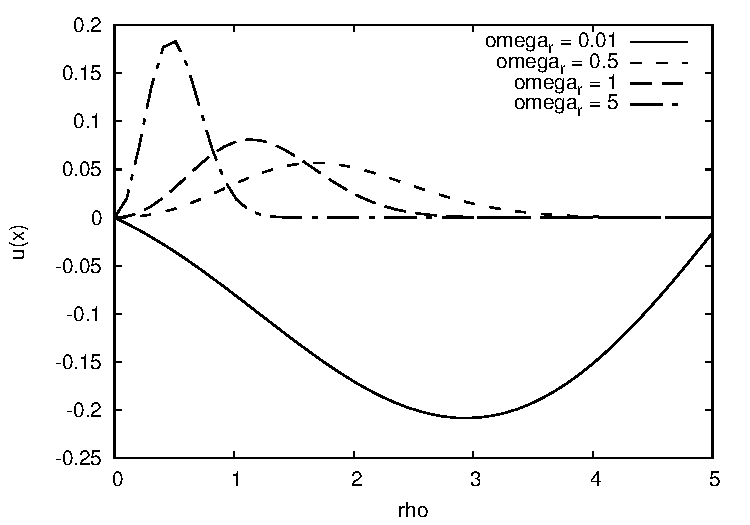
\includegraphics{waveplot}
	\caption{Wave functions of the lowest energy state for $\omega_r = 0.01$, $\omega_r = 0.5$, $\omega_r = 1$ and $\omega_r = 5$.}
	\label{fig:wave}
\end{figure}

\begin{figure}[h]
	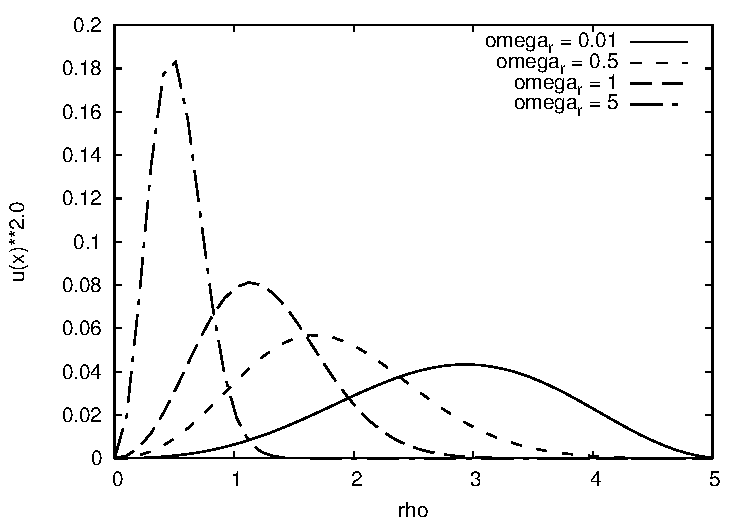
\includegraphics{waveplotabs}
	\caption{Probability distribution of the lowest energy state for $\omega_r = 0.01$, $\omega_r = 0.5$, $\omega_r = 1$ and $\omega_r = 5$.}
	\label{fig:waveabs}
\end{figure}


\section{Analysis of results}

The larger $n$ we used the more of a difference there was between the smallest eigenvalues from the Armadillo function and our Jacobi algorithm (that is based on the one in the lecture notes). So something is obviously very wrong.

In theory the number of iterations/rotations should be something like $3n^2 - 5n^2$, but we get a small amount and the difference seem to increase almost linearly with $n$. We have no idea why this happens but it is probably related to why our eigenvalues also become ``more wrong'' the larger $n$ is.

Looking at figure ~\ref{fig:waveabs}, the Coloumb force between the electrons becomes weaker when we move away from the bottom of the oscillator potential, and the oscillator potential becomes stronger. The stronger the oscillator potential is (higher $\omega_r$) the more that potential push the particles together. While when the oscillator potential is weak (low $\omega_r$) the Coloumb force is large than the force from the oscillator potential until a larger distance between the electrons. The plot confirms this.

When we increase $\omega_r$ the lowest eigenvalue increases, that is the energy in the ground state increases. This is because the particles are further up the Coloumb potential (as this potential doesn't change with $\omega_r$ and the oscillator potential becomes stronger).

Note: We discovered last minute that in our program we had ``\texttt{A(i,l) = c*a\_il + s*a\_il;}'' instead of ``\texttt{A(i,l) = c*a\_il + s*a\_ik;}''. However, changing this did not really help much. Due to time constraints we could not resolve the problem, and the plots shown in this report are therefore made using Armadillos eigenvalue/eigenvector function. 

\section{Repository}
The repository where you can find our programs is at \url{https://github.com/miktoki/FYS3150}.

%\bibliographystyle{plain}
%\bibliography{refs}

%\printindex
\end{document}


